%
% Recomendaciones del NIST para la administración de llaves,
% capítulo de análisis y diseño para la generación de tokens.
% Proyecto Lovelace
%

\capitulo{Administración de llaves}{sec:administracion_llaves}
{
  \epigrafe
  {%
    Cangrejo: ... un maravilloso concierto de piano para dos manos izquierdas.
    El penúltimo (y único) movimiento era una fuga a una voz. No puede imaginar
    lo intrincada que era. Como finale, tocamos la novena Zenfonía de Beethoven.
    Cuando terminó, toda la audiencia se puso de pie y aplaudió con una mano.
    Fue sobrecogedor.
  }
  {%
    Gödel, Escher, Bach: An Eternal Golden Braid, Contrafactus,
    \textsc{Douglas R. Hofstadter}.%
  }
}

\section{Tipos de llaves}

En \cite{nist_llaves}, el \gls{gl:nist} divide a las llaves criptográficas en
19 categorías, las cuales surgen de la combinación de la naturaleza de la
llave (simétrica, pública o privada) con la funcionalidad que se le da
(firmas, autenticación, cifrado, entre otras). En la tabla
\ref{clasificacion_llaves} se muestran dichas categorías: se marca con
$ \checkmark $ las combinaciones que tienen sentido práctico; por ejemplo, para
firmar (y posteriormente validar) solamente se ocupan las llaves de un esquema
asimétrico (i. e. públicas y privadas).

\begin{description}

  \item[Para firmas:] llaves que son usadas en algoritmos asimétricos para
    generar firmas digitales con posibles implicaciones a largo plazo. Cuando
    son manejadas correctamente, este tipo de llaves está diseñado para
    proveer \gls{gl:autenticacion_origen}, autenticación de integridad y
    soporte para el no repudio.

  \item[Para autenticación:] son usadas para proporcionar garantías sobre la
    identidad de un fuente generadora (i. e. \gls{gl:autenticacion_origen}).

  \item[Para cifrado de datos:] usadas en esquemas simétricos para proveer de
    confidencialidad a la información (esto es, para cifrar la información).
    Como se tratan de algoritmos simétricos (o de llave secreta), la misma
    llave se usa para quitar la confidencialidad (para descifrar).

  \item[Como envoltura de otras llaves:] también llamadas llaves cifradoras de
    llaves (\textit{key-encrypting keys}), son usadas para proteger otras
    llaves usando algoritmos simétricos. Dependiendo del algoritmo con el que
    se use la llave, esta también puede ser usada para proveer de validaciones
    de integridad.

  \item[Para generadores aleatorios:] llaves usadas para generar números o bits
    aleatorios.

  \item[Como llaves maestra:] una llave maestra simétrica se usa para derivar
    otras llaves simétricas (p. ej. llaves de cifrado, o de envoltura). También
    se conoce como llave de derivación de llaves (\textit{key-derivation key}).

  \item[Para el transporte de llaves:] llaves utilizadas en esquemas
    asimétricos para proteger la comunicación en un proceso de acuerdo de
    llaves. Se usan para proteger otras llaves (p. ej. de cifrado, de
    envoltura) o información relacionada (p. ej.
    \glspl{gl:vector_de_inicializacion}).

  \item[Para el acuerdo de llaves:] utilizadas en algoritmos de acuerdo de
    llaves para establecer otras llaves. Generalmente funcionan en plazos muy
    largos.

  \item[Efímeras para el acuerdo de llaves:] llaves de muy corto plazo que son
    usadas una sola vez en un proceso de establecimiento de otras llaves. En
    algunos casos la llave efímera puede ser usada más de una vez, pero dentro
    de la misma transacción.

  \item[De autorización:] usadas para proveer y verificar los privilegios de
    una entidad. En un esquema simétrico, la llave es conocida tanto por la
    entidad que provee acceso, como por la que desea acceder.

\end{description}

%Además de las llaves, existen algunos otros parámetros que comunmente se usan
%en los algoritmos criptográficos, y que también necesitan ser tomados en
%consideración:
%
%\begin{description}
%
%  \item[Parámetros de dominio:] Son usados junto con algunos algoritmos de
%    llave pública para generar pares de llaves o crear firmas digitales.
%
%  \item[\glspl{gl:vector_de_inicializacion}:] usados en algunos
%    \glspl{gl:modo_de_operacion} (ver el glosario).
%
%  \item[Secretos compartidos:] son generados durante el proceso de acuerdo de
%    llaves. Estos deben ser manejados y protegidos de la misma forma que las
%    llaves criptográficas.
%
%  \item[Semillas de \gls{gl:rng}:] son usadas en la generación de números
%    aleatorios determinísticos.
%
%  \item[Otros datos públicos:] información pública extra que es usada durante
%    el proceso de establecimiento de llaves (por ejemplo los \textit{nonce}).
%
%  \item[Otros datos privados:] información secreta usada en el proceso de
%    establecimeinto de llaves (por ejemplo una semilla de un \gls{gl:rng}).
%
%  \item[Resultados intermedios:] resultados intermedios de operaciones
%    criptográficas; estos deben ser protegidos, y no deben ser usados de una
%    manera distinta a la establecida por el algoritmo criptgráfico.
%
%  \item[Información de control de llaves:] información relacionada al material
%    de llaves (\textit{keying material}), por ejemplo, el identificador, un
%    propósito, un contador, etcétera; se debe de proteger para poder asegurar
%    que esta información puede ser usada correctamente. La información de
%    control de llaves se debe incluir en los metadatos de una llave.
%
%  \item[Números aleatorios:] los números creados por un \gls{gl:rng} se deben
%    de proteger cuando se retengan.
%
%  \item[Contraseñas:] las contraseñas son usadas para adquirir privilegios de
%    acceso, y pueden ser usadas como credenciales en mecanismos de
%    \gls{gl:autenticacion_origen}. Las contraseñas también se pueden usar para
%    derivar llaves criptográficas que son usadas para protejer y acceder
%    a contenido alamcenado.
%
%  \item[Información de auditoría:] la infromación de auditorías contiene
%    registros de los eventos de la administración de llaves.
%
%\end{description}

\section{Usos de llaves}

En general, las llaves se deben de utilizar para un solo propósito: el uso de
la misma llave para dos operaciones criptográficas puede debilitar la seguridad
provista por ambas; al limitar el uso de una llave se limita el nivel de riesgo
de que esta se vea comprometida; algunos usos de llaves interfieren unos
con otros.

La regla anterior no se extiende a situaciones en donde el mismo
proceso provea de múltiples servicios. Por ejemplo, cuando una sola firma
digital provee de autenticación de integridad y de autenticación de origen,
o cuando una sola llave simétrica es usada para cifrar y para autenticar en
una sola operación.

\begin{table}
  \centering
  \begin{tabular}{| c | l | c | c | c |}

    \cline{3-5}
    \multicolumn{2}{c |}{} &
    \multicolumn{3}{ c |}{\textbf{Naturaleza}} \\
    \cline{3-5}
    \multicolumn{2}{c |}{} &
    Simétrica &
    Pública &
    Privada \\
    \hline

    \multirow{10}{*}{\begin{sideways} \textbf{Funcionalidad} \end{sideways}}
    & Para firmas                        &            & \checkmark & \checkmark
    \\\cline{2-5}
    & Para autenticación                 & \checkmark & \checkmark & \checkmark
    \\\cline{2-5}
    & Para cifrado de datos              & \checkmark &            &
    \\\cline{2-5}
    & Como envoltura de otras llaves     & \checkmark &            &
    \\\cline{2-5}
    & Para generadores aleatorios        & \checkmark &            &
    \\\cline{2-5}
    & Como llave maestra                 & \checkmark &            &
    \\\cline{2-5}
    & Para el transporte de llaves       &            & \checkmark & \checkmark
    \\\cline{2-5}
    & Para el acuerdo de llaves          & \checkmark & \checkmark & \checkmark
    \\\cline{2-5}
    & Efímeras para el acuerdo de llaves &            & \checkmark & \checkmark
    \\\cline{2-5}
    & De autorización                    & \checkmark & \checkmark & \checkmark
    \\\hline

  \end{tabular}
  \caption{Clasificación de llaves criptográficas}
  \label{clasificacion_llaves}
\end{table}

\section{Criptoperiodos}

Un criptoperiodo es el rango de tiempo durante el cual una llave es válida.
Algunas de las funciones de los criptoperiodos son:

\begin{itemize}

  \item Limitar el total de daños si una sola llave se ve comprometida.

  \item Limitar el uso de un algoritmo en particular (\textit{particular}
    en el sentido de la instancia misma del algoritmo).

  \item Limitar el tiempo disponible para intentos de ataques sobre los
    mecanismos que protegen a la llave del acceso sin autorización.

  \item Limitar el periodo en el cual la información puede verse comprometida
    por revelaciones inadvertidas de llaves a entidades sin autorización.

  \item Limitar el tiempo disponible para ataque criptoanalíticos.

\end{itemize}

A continuación se enlistan los principales factores a tomar en cuenta al
momento de establecer un criptoperiodo:

\begin{itemize}

  \item La fuerza del mecanismo criptográfico (el algoritmo, la
    \gls{gl:fuerza_efectiva} de la llave, el tamaño de bloque, el modo de
    operación, etc.).

  % ¿La encarnación de los mecanismos?

  \item El entorno de operacion (p. ej. un lugar de acceso restringido, una
    terminal pública).

  \item El volumen de información transmitida, o el número de transacciones.

  \item La función de seguridad (cifrado de datos, firma digital, derivación
    de llaves, etc.).

  \item El método de entrada de la llave (por teclado, a nivel de sistema).

  \item El número de nodos en una red que comparten la misma llave.

  \item El número de copias de la llave distribuidas.

  \item Rotaciones de personal.

  \item La amenaza de los adversarios (¿de quién se está protegiendo la
    información?, ¿cuáles son sus capacidades?)

  \item La amenza de avances tecnológicos (nuevos límites para el problema
    del logaritmo discreto, computadoras cuánticas).

\end{itemize}

La duración de los criptoperiodos también debe tomar en cuenta cuáles son
los riesgos de las actualizaciones de llaves. En general, entre más cortos
sean los criptoperiodos, mejor; sin embargo, si los mecanismos de distribución
de llaves son manuales y propensos a errores humanos, entonces el riesgo se
invierte. En estos casos (en especial cuando se utiliza
\gls{gl:criptografia_fuerte}) resulta mejor tener pocas y bien controladas
distribuciones manuales, a que estas sean frecuentes y mal controladas.

Las consecuencias de una exposición se miden de acuerdo a qué tan sensible es
la información, qué tan críticos son los procesos protegidos, y qué tan alto
es el costo de recuperación en caso de exposición. La sensibilidad se refiere
al periodo de tiempo durante el cual la información debe estar protegida (5
segundos, 5 minutos, 5 horas o 5 años) y a las consecuencias potenciales en
caso de pérdida de protección. En general, entre más sensible sea la
información protegida, el criptoperiodo debe ser menor (sin llegar a que
sea contraproducente).

Algunos otros factores a tomar en cuenta incluyen el uso de las llaves y el
costo de actualizaciones. En cuanto al uso de las llaves, generalmente se
hace distinción en cuanto a si la información protegida solamente se está
transfiriendo, o si se va a almacenar; en general los criptoperiodos son más
largos en caso de almacenamiento, dado el costo que puede representar el
recifrado de toda una base de datos. Esto está relacionado con el costo de
las actualizaciones: cuando el volumen de información protegida es demasiado
grande o cuando esta se encuentra distribuida en distintos puntos geográficos,
el costo de un cambio de llaves puede ser demasiado elevado.

La tabla \ref{criptoperiodos_sugeridos} muestra las sugerencias del
\gls{gl:nist} en \cite{nist_llaves} en cuanto a la duración de los
criptoperiodos según cada tipo de llave.

\begin{table}
  \centering
  \begin{tabular}{| p{0.5\textwidth} | P{0.2\textwidth} | P{0.2\textwidth} |}

    \hline
    \multirow{2}{*}{\textbf{Tipo de llave}} &
    \multicolumn{2}{ c |}{\textbf{Criptoperiodo}} \\
    \cline{2-3}
    & \textbf{Periodo de uso de emisor (PE)}
    & \textbf{Periodo de uso de receptor (PR)} \\
    \hline

    1.- Llave privada para firma &
    1 a 3 años &
    - \\
    \hline

    2.- Llave pública para verificación de firma &
    \multicolumn{2}{ c |}{Depende del tamaño de la llave} \\
    \hline

    3.- Llave simétrica para autenticación &
    $ \leq 2 $ años &
    $ \leq PE + 3 $ años \\
    \hline

    4.- Llave privada para autenticación &
    \multicolumn{2}{ c |}{1 a 2 años} \\
    \hline

    5.- Llave pública para autenticación &
    \multicolumn{2}{ c |}{1 a 2 años} \\
    \hline

    6.- Llave simétrica para cifrado de datos &
    $ \leq 2 $ años &
    $ \leq PE + 3 $ años \\
    \hline

    7.- Llave simétrica como envoltura &
    $ \leq 2 $ años &
    $ \leq PE + 3 $ años \\
    \hline

    8.- Llave simétrica para generadores aleatorios &
    ver SP800-90 &
    - \\
    \hline

    9.- Llave simétrica maestra &
    alrededor de 1 año &
    - \\
    \hline

    10.- Llave privada para transporte &
    \multicolumn{2}{ c |}{$ \leq 2 $ años} \\
    \hline

    11.- Llave pública para transporte &
    \multicolumn{2}{ c |}{1 a 2 años} \\
    \hline

    12.- Llave simétrica para acuerdo &
    \multicolumn{2}{ c |}{1 a 2 años} \\
    \hline

    13.- Llave privada para acuerdo &
    \multicolumn{2}{ c |}{1 a 2 años} \\
    \hline

    14.- Llave pública para acuerdo &
    \multicolumn{2}{ c |}{1 a 2 años} \\
    \hline

    15.- Llave privada efímera para acuerdo &
    \multicolumn{2}{ c |}{Solo 1 transacción} \\
    \hline

    16.- Llave pública efímera para acuerdo &
    \multicolumn{2}{ c |}{Solo 1 transacción} \\
    \hline

    17.- Llave simétrica para autorización &
    \multicolumn{2}{ c |}{$ \leq 2 $ años} \\
    \hline

    18.- Llave privada para autorización &
    \multicolumn{2}{ c |}{$ \leq 2 $ años} \\
    \hline

    19.- Llave pública para autorización &
    \multicolumn{2}{ c |}{$ \leq 2 $ años} \\
    \hline

  \end{tabular}
  \caption{Criptoperiodos sugeridos por tipo de llave}
  \label{criptoperiodos_sugeridos}
\end{table}

% Demasiado abstracto:
%
%\section{Garantías}
%
%Cuando una llave es almacenada o distribuida, podría pasar por entornos
%inseguros; es por esto por lo que antes de usarse para sus operaciones
%criptográficas normales, una llave debe cumplir con las siguientes garantías.
%
%\begin{description}
%
%  \item[Garantía de integridad:] como mínimo, la integridad se debe obtener
%    verificando que el material de la llave tiene el formato correcto y
%    proviene de fuentes autorizadas. De manera adicional se pueden usar
%    códigos de detección de error, códigos de autenticación de mensaje y
%    firmas digitales.
%
%  \item[Garantía de validez de parámetros de dominio:] los parámetros de
%    dominio son usados por los algoritmos de llave pública al momento de la
%    generación de llaves y firmas digitales, y durante la generación de
%    secretos compartidos. Esta garantía es muy importante, y se debe obtener
%    antes de usar el algoritmo.
%
%  \item[Garantía de validez de llave pública:] esta validación permite al
%    usuario estar seguro de que la llave pública es aritméticamente correcta.
%    Esto reduce las posibilidades de usar llaves débiles o corruptas. Una de
%    varias maneras de obtener esta garantía es mediante la verificación de
%    algunas propiedades matemáticas que la llave pública debe tener (estas
%    dependen según el algoritmo).
%
%  \item[Garantía de posesión de llave privada:] esta garantía debe ser obtenida
%    por ambas partes: el dueño de los pares y las demás entidades que
%    reciben la llave pública. Los métodos para obtener la garantía son
%    específicos a cada algoritmo.
%
%\end{description}

\section{Estados de llaves y transiciones}

En la figura \ref{estados_de_llaves} se muestra un diagrama de estados con
los posibles comportamientos de una llave criptográfica. Un criptoperiodo
inicia al entrar en el estado «activo» (transición 4) y termina al llegar al
estado «destruido». En el caso de esquemas asimétricos, las transiciones se
aplican a ambos pares de llaves. Se debe llevar un registro de la fecha y hora
(y en algunos casos de las razones) de cualquier cambio de estado.

\begin{figure}
  \begin{center}
    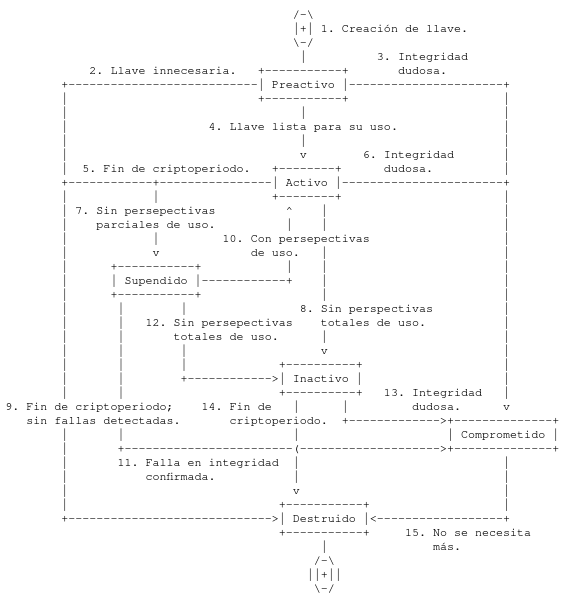
\includegraphics[width=0.8\linewidth]{diagramas/estados_de_llaves_ascii.png}
    \caption{Diagrama de estado de llaves criptográficas.}
    \label{estados_de_llaves}
  \end{center}
\end{figure}

Hay varias posibles razones por las que se puede llegar a un estado
«suspendido»: la entidad dueña de una firma digital no se encuentra disponible;
se sospecha que la integridad de la llave está comprometida, por lo que se pasa
a este estado en lo que se investiga más en profundidad; entre otros. Una
llave que está en este estado («suspendido») no debe ser usada bajo ninguna
circunstancia.

Las llaves que se encuentran en el estado «inactivo» no deben ser usadas para
aplicar protección criptográfica, pero en algunos casos, pueden ser usadas
para procesar información protegida con criptografía. Por ejemplo, las llaves
simétricas usadas para autenticación, cifrado de datos o envoltura de llaves,
pueden ser usadas para procesar información hasta que acabe el periodo del
emisor de la llave emisora.

El estado «comprometido» representa a las llaves a las que una entidad sin
autorización tiene o ha tenido acceso. Las llaves comprometidas no deben ser
usadas para aplicar protección criptográfica, sin embargo, en algunos casos
es posible que sean usadas para procesar información (en condiciones
sumamente controladas); por ejemplo, si la cierta información fue firmada
antes de que se produjera la brecha de seguridad, las llaves pueden ser
usadas para valida esta firma.
